\documentclass[12pt]{beamer}
\usepackage{tikz}
\usepackage{booktabs}
\usepackage{graphicx}
\usepackage{subcaption}

\title[EM2091]{Review and matlab implementation of the paper:} % Text in square brackets is displayed in the footer
\subtitle{\textit{Using neural network ensembles for bankruptcy prediction and credit scoring (Tsai, Wu)}}
\author[Filippo Tolin]{
    \href{mailto:874631@stud.unive.it}{Filippo Tolin}
}
\institute[Ca' Foscari]{Ca' Foscari University of Venice }
\date{March 28, 2024}


\usepackage{template}


\begin{document}
\begin{frame}
\titlepage
\end{frame}

\begin{frame}{Summary}
\tableofcontents 
\end{frame}

\section{Paper review}

\subsection{Goals}

\begin{frame}{Goals}
  \begin{itemize}
    \item Observe the performance differences between different ANN ensemble
      approaches, namely single classifiers,
      multiple classifiers and diversified multiple classifiers, with regards to based on a set
      credit scoring and bankruptcy detection. The study is based on three
      of heterogeneous datasets;
    \item Evaluate the three classifier architectures performance with regards to
      Type 1 error and Type 2 error.
  \end{itemize}
\end{frame}

\subsection{Tools}

\begin{frame}{Tools}
  \begin{itemize}
    \item Multilayer Perceptron feedforward Artificial Neural Network
      \begin{itemize}
        \item One \textbf{hidden} layer
        \item Five different values for the \textbf{hidden nodes} hyperparameter
        \item Four different values for the \textbf{training epochs} hyperparameter
      \end{itemize}
    \item Multiple classifiers with two techniques to compute them:
      \begin{enumerate}
        \item Best $n$ classifiers for every epoch
        \item Best $n$ classifiers among all the epochs
      \end{enumerate}
      \begin{block}{Note}
        Technique $1$ is only applicable to $n=3 \wedge n=5$,
        with $n \in [3,5,7,9,11,13,15]$. Multiple classifiers are based on \textbf{majority voting}.
      \end{block}
  \end{itemize}
\end{frame}

\subsection{Advancements vs previous works}

\begin{frame}{Advancements vs previous works}
  \begin{itemize}
    \item Employment of \textbf{multiple datasets} for system validation;
    \item Usage of \textbf{Type 1 and Type 2 errors} and not only average accuracy measures;
    \item Testing the classifiers performance on multiple classification tasks
      rather than a single one, specifically on \textbf{credit scoring} and \textbf{bankruptcy prediction}.
  \end{itemize}
\end{frame}

\begin{frame}{Brief remark}
\begin{itemize}
\item \textbf{Type 1} error is associated with \textbf{false positives};
\item \textbf{Type 2} error is associated with \textbf{false negatives}.
\end{itemize}

\begin{examples}
  \begin{itemize}
    \item \textit{Type 1}: the model classifies a credit-worthy client as a credit-risky one;
    \item \textit{Type 2}: the model classifiers a credit-risky client as a credit-worthy one.
  \end{itemize}
\end{examples}

\end{frame}

\subsection{Study 1,2,3}

\begin{frame}{Study 1: single vs multiple classifiers}
  \begin{itemize}
    \item Datasets are split into training (70\%) and test (10\%);
    \item For single classifiers the number of nodes is $nn \in [8,12,16,24,32]$
      and learning epochs $[50,100,200,300]$.
    \item Multiple classifers are build with the voting strategy combining the results
      of the top $n$ classifers, with $n \in [3,5,7,9,11,13,15]$.
  \end{itemize}
  \begin{block}{Takeout}
  On average, the single best classifer outperforms multiple classifers.
  \end{block}
\end{frame}

\begin{frame}{Study 1: single vs multiple classifiers}
  \begin{figure}
    \centering
    \subcaptionbox{Australian\label{fig:st1aus}}{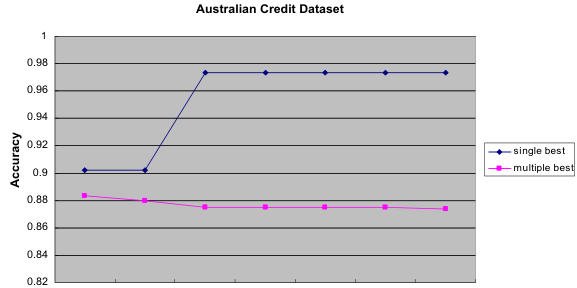
\includegraphics[width=0.41\linewidth]{images/st1aus.png}}\hfill
    \subcaptionbox{German\label{fig:st1ger}}{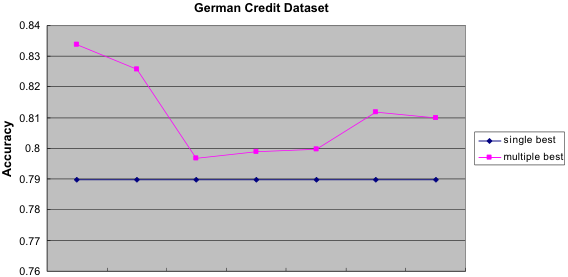
\includegraphics[width=0.41\linewidth]{images/st1ger.png}}\hfill
    \subcaptionbox{Japanese\label{fig:st1jap}}{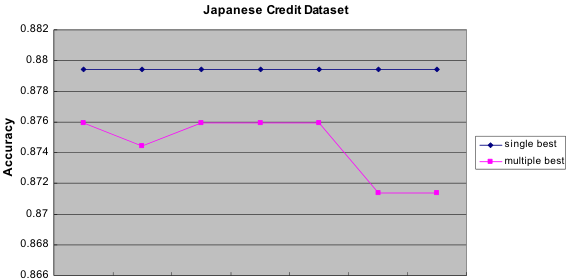
\includegraphics[width=0.41\linewidth]{images/st1jap.png}}
    \caption{Comparison between single classifiers and multiple classifiers.}
\end{figure}
\end{frame}



\begin{frame}{Study 2: single vs multiple vs diversified classifiers}
  \begin{itemize}
    \item Train-test dataset generation is different for diversified multiple classifiers.
      Specifically, every model composing
      the classifier is trained on a fraction of the observations from the same
      dataset, then the majority
      voting is executed using a test dataset;
    \item The procedure aims at ensuring \textbf{diversity} between classifiers.
  \end{itemize}

  \begin{block}{Takeout}
    The best single classifier is still, on average, a better classifier than
    the diversified multiple classifier (and the multiple classifier, as seen before).
  \end{block}

\end{frame}

\begin{frame}{Study 2: single vs multiple vs diversified classifiers}
  \begin{figure}
    \centering
    \subcaptionbox{Australian\label{fig:st2aus}}{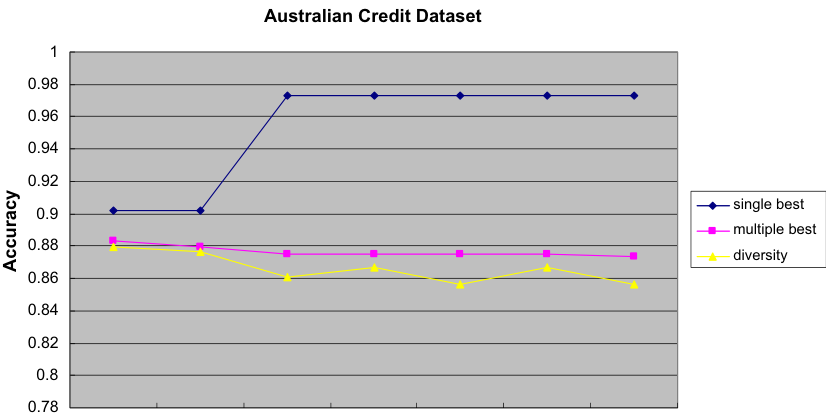
\includegraphics[width=0.40\linewidth]{images/st2aus.png}}\hfill
    \subcaptionbox{German\label{fig:st2ger}}{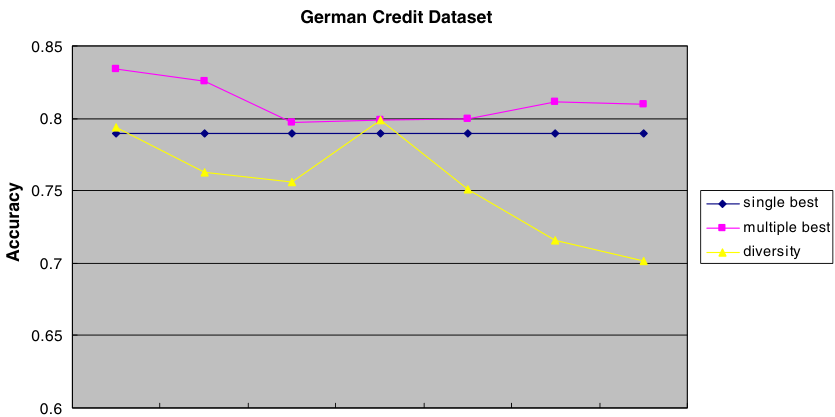
\includegraphics[width=0.40\linewidth]{images/st2ger.png}}\hfill
    \subcaptionbox{Japanese\label{fig:st2jap}}{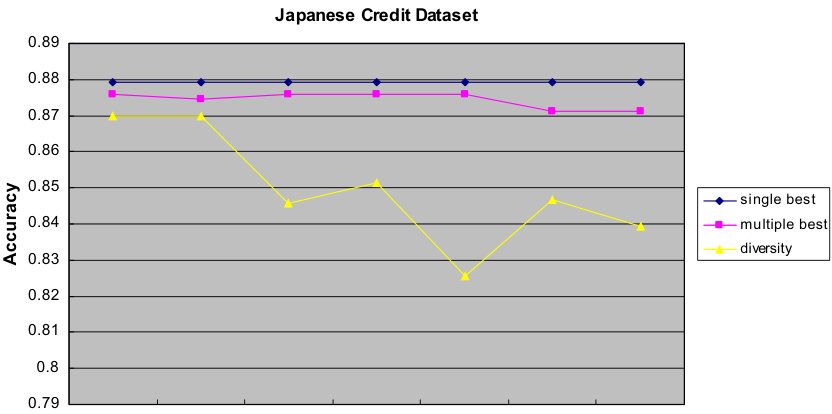
\includegraphics[width=0.40\linewidth]{images/st2jap.png}}
    \caption{Comparison between single, multiple and diversified classifiers.}
\end{figure}
\end{frame}



\begin{frame}{Study 3: Type 1 and Type 2 errors}
  \begin{itemize}
    \item In Study 1 and Study 2 the results of classifiers are compared based on
      the \textbf{accuracy} of the classifiers. Study 3 compares the models
      performance with regards to Type 1 and Type 2 errors.
  \end{itemize}

  \begin{block}{Takeout}
    This study highlights how single classifiers do not totally outperform multiple
    or diversified classifiers.
  \end{block}
\end{frame}

\begin{frame}{Study 3: Type 1 and Type 2 errors}
  \begin{figure}
    \centering
    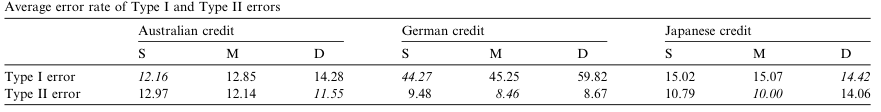
\includegraphics[width=1\linewidth]{images/error.png}
    \caption{Type 1 and Type 2 error across datasets and classifier architectures.}
\end{figure}
\end{frame}

\subsection{Conclusions}

\begin{frame}{Conclusions}
  \begin{itemize}
    \item If the performance is measured with \textbf{accuracy}, \textbf{single best neural
      network classifier is more suitable} for bankruptcy
      prediction and credit scoring tasks, if compared with multiple or diversified
      multiple neural network classfiers;
    \item If performance is measured with \textbf{type 1 and 2 errors}, there seems
      to be no \textbf{clear winner} among the model architectures analysed.
  \end{itemize}
\end{frame}

\section{A couple of remarks\dots}

\begin{frame}{A couple of remarks\dots}
  \begin{itemize}
    \item The methodology used to build the datasets for diversified multiple classifers
      could be associated with the poor performance by the classifiers. In fact
      the higher the $n$ the smaller the train-sets used for each models' training.
      This could lead to a lot of results variability;
    \item It's not clear why the authors used two methodologies to build the multiple
      classifiers even though one of them is applicable only to $n=3$ and $n=5$
      classifiers.
  \end{itemize}
\end{frame}

%------------------------------------------------
\section{Matlab implementation}
%------------------------------------------------

\subsection{Methodology}



\subsection{Model}

\subsection{Single classifier}

\subsection{Multiple classifier}

\subsection{Diversified multiple classifier}

\subsection{Results of Study 1 and 2}

\subsection{Type 1 and 2 error}
\begin{frame}{Type 1 and 2 error: setup}
\begin{itemize}
  \item \textbf{Single classifier}
  \item \textbf{Multiple classifier}
\end{itemize}
\end{frame}

\begin{frame}{Type 1 and 2 error: results}
  
\end{frame}

\subsection{Conclusions}




%------------------------------------------------

\begin{frame}[fragile] % Need to use the fragile option when verbatim is used in the slide
    \frametitle{Citation}
    An example of the \verb|\cite| command to cite within the presentation:\\~

    %This statement requires citation \cite{p1}.
\end{frame}

%------------------------------------------------

\begin{frame}{References}
    % Beamer does not support BibTeX so references must be inserted manually as below
    \footnotesize{
        \begin{thebibliography}{99}
            \bibitem[Smith, 2012]{p1} John Smith (2012)
            \newblock Title of the publication
            \newblock \emph{Journal Name} 12(3), 45 -- 678.
        \end{thebibliography}
    }
\end{frame}

%------------------------------------------------

\begin{frame}
    \Huge{\centerline{The End}}
\end{frame}

%----------------------------------------------------------------------------------------


\end{document}
